\documentclass{report}
\usepackage{graphicx}
\usepackage{pgfplots}
\begin{document}
\begin{titlepage}
\centering
{\bfseries\LARGE Instituto Tecnol\'ogico de Costa Rica \par}
\vspace{1cm}
{\scshape\Large Facultad de Ingenier\'ia en Computaci\'on \par}
\vspace{3cm}
{\scshape\Huge Simulaci\'on de propagaci\'on \\
de CODEVID-19\par}
\vspace{3cm}
{\itshape\Large Proyecto 2\par}
\vfill
{\Large Emanuelle Jim\'enez S.\par}
{\Large Fabrizio Alvarado B.\par}
\vfill
{\Large Junio 2020 \par}
\end{titlepage}
\newpage
\section{Gr\'afico}
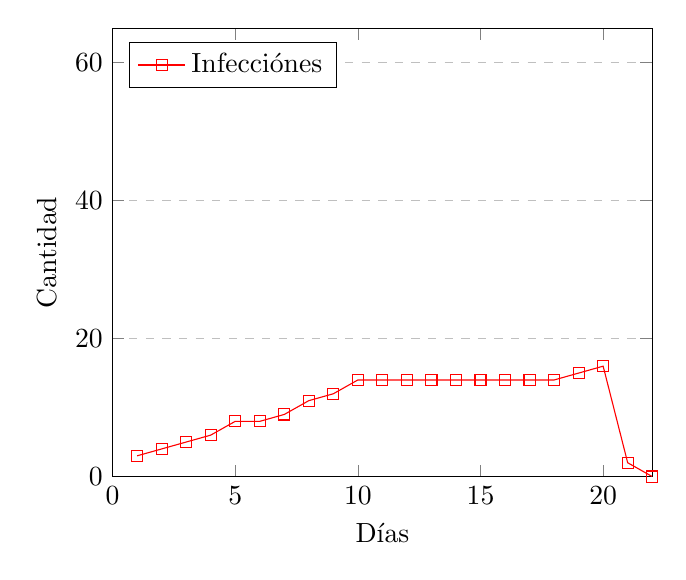
\begin{tikzpicture}
\begin{axis}[
xlabel={D\'ias},
ylabel={Cantidad},
xmin=0, xmax=22,
ymin=0, ymax=65,
legend pos=north west,
ymajorgrids=true,
grid style=dashed,
]
\addplot[
color=red,
mark=square,
]
coordinates {
(1, 3)(2, 4)(3, 5)(4, 6)(5, 8)(6, 8)(7, 9)(8, 11)(9, 12)(10, 14)(11, 14)(12, 14)(13, 14)(14, 14)(15, 14)(16, 14)(17, 14)(18, 14)(19, 15)(20, 16)(21, 2)(22, 0)
};
\legend{Infecci\'ones}
\end{axis}
\end{tikzpicture}
\newpage
\section{Cambios en el mapa}
\includegraphics[scale=0.20]{1}
\includegraphics[scale=0.20]{2}
\includegraphics[scale=0.20]{3}
\includegraphics[scale=0.20]{4}
\includegraphics[scale=0.20]{5}
\includegraphics[scale=0.20]{6}
\includegraphics[scale=0.20]{7}
\includegraphics[scale=0.20]{8}
\includegraphics[scale=0.20]{9}
\includegraphics[scale=0.20]{10}
\includegraphics[scale=0.20]{11}
\includegraphics[scale=0.20]{12}
\includegraphics[scale=0.20]{13}
\includegraphics[scale=0.20]{14}
\includegraphics[scale=0.20]{15}
\includegraphics[scale=0.20]{16}
\includegraphics[scale=0.20]{17}
\includegraphics[scale=0.20]{18}
\includegraphics[scale=0.20]{19}
\includegraphics[scale=0.20]{20}
\includegraphics[scale=0.20]{21}
\end{document}
